\documentclass[solution, letterpaper]{cs121}

\usepackage{graphicx}

%% Please fill in your name and collaboration statement here.
%\newcommand{\studentName}{Renzo Lucioni and Daniel Broudy}
%\newcommand{\collaborationStatement}{I collaborated with...}
\newcommand{\solncolor}{red}
\begin{document}

\header{1}{March 5, 2013, at 11:40 AM}{}{}

%%%%%%%%%%%%%%%%%%%%%%%%%%%%%%%%%%%%%%%%%%%%%%%%%%%%
\section*{Quantitative Results}
\subsection*{Dimension 0 - Weights Assigned Randomly}

The following is a graph showing the average tree size over 5 trials for several values of $n$: 
\begin{center}
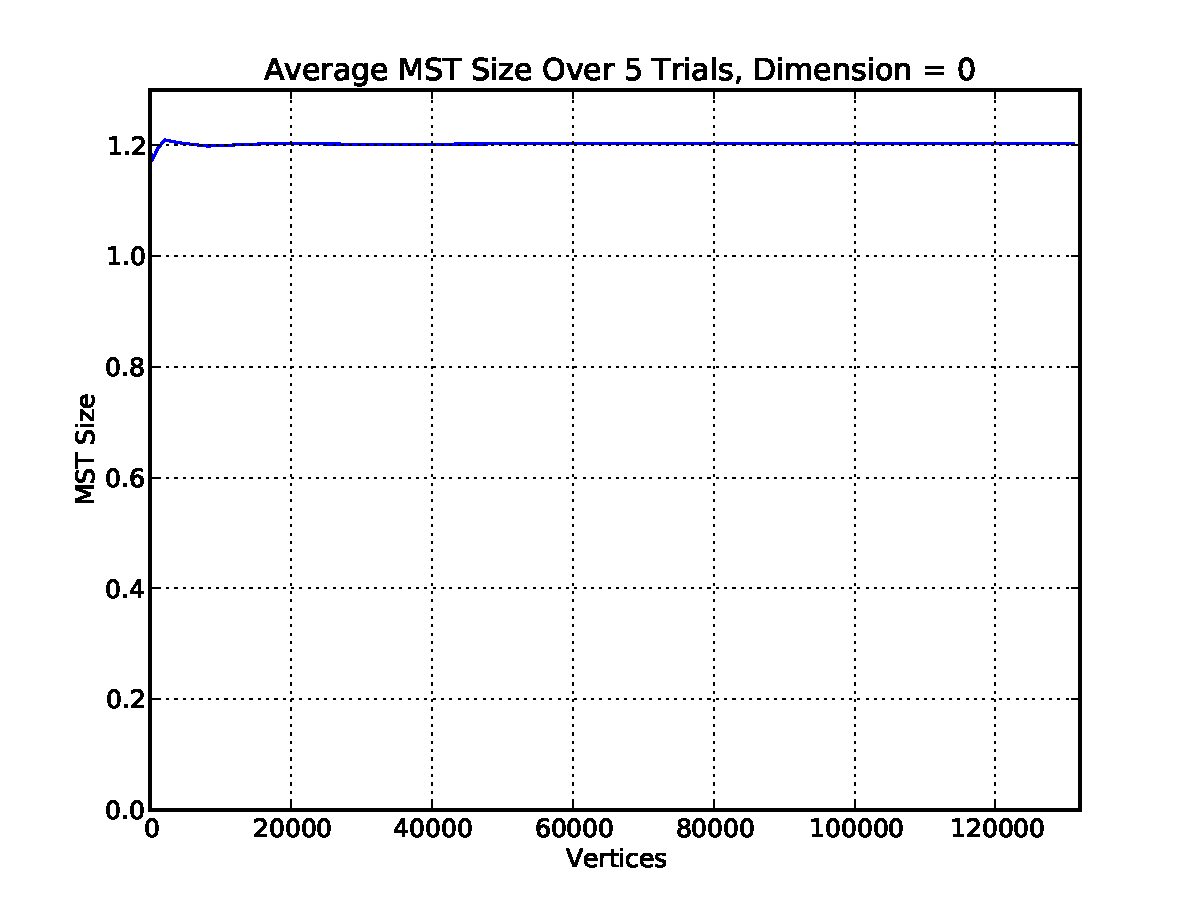
\includegraphics[scale=0.6]{graphs/kruskals-dimension-0.pdf}
\begin{tabular}{ | r | l |}
\hline
\bf{\itshape{n}} & \bf{Avg. MST Weight} \\
\hline
16 & 0.929531 \\
\hline
32 & 0.967641 \\
\hline
64 & 1.137753 \\
\hline
128 & 1.185701 \\
\hline
256 & 1.173584 \\
\hline
512 & 1.178243 \\
\hline
1024 & 1.192734 \\
\hline
2048 & 1.209832 \\
\hline
4096 & 1.204681 \\
\hline
8192 & 1.198778 \\
\hline
16384 & 1.203032 \\
\hline
32768 & 1.202110 \\
\hline
65536 & 1.203110\\
\hline
131072 & 1.203856\\
\hline
\end{tabular}
\end{center}

A simple function that describes the above plot is $f(n) \approx 1.2$

\subsection*{Dimension 2 - Unit Square}

The following is a graph showing the average tree size over 5 trials for several values of $n$:
\begin{center}
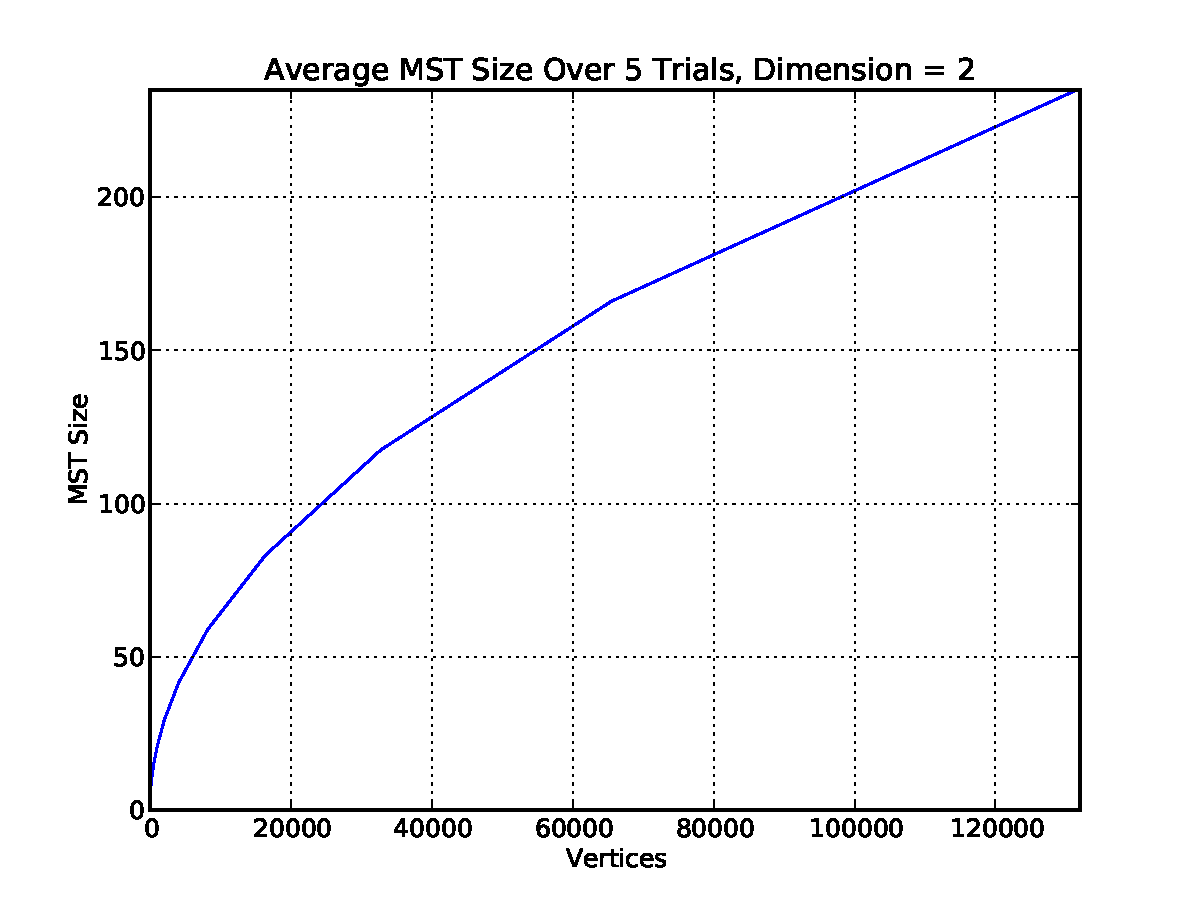
\includegraphics[scale=0.6]{graphs/kruskals-dimension-2.pdf}
\begin{tabular}{ | r | l |}
\hline
\bf{\itshape{n}} & \bf{Avg. MST Weight} \\
\hline
16 & 2.818149 \\
\hline
32 & 3.872131 \\
\hline
64 & 5.475579 \\
\hline
128 & 7.691335 \\
\hline
256 & 10.648638 \\
\hline
512 & 14.866658 \\
\hline
1024 & 20.792080 \\
\hline
2048 & 29.512669 \\
\hline
4096 & 41.692554 \\
\hline
8192 & 58.925728 \\
\hline
16384 & 83.156471\\
\hline
32768 & 117.546494\\
\hline
\end{tabular}
\end{center}

This curve is best described by a function of the form $f(n)=an^b$, where $a > 0$ and $\frac{1}{2} \leq b \leq 1$. Using Mathematica's {\tt FindFit} function in conjunction with the data used to generate the above graph, we achieved $a=0.647963$ and $b=0.50009$ as the best fit values for this function, giving us the following best guess for $f(n)$:
\[f(n) \approx 0.65 n^{\frac{1}{2}}\]

\pagebreak

\subsection*{Dimension 3 - Unit Cube}

The following is a graph showing the average tree size over 5 trials for several values of $n$:
\begin{center}
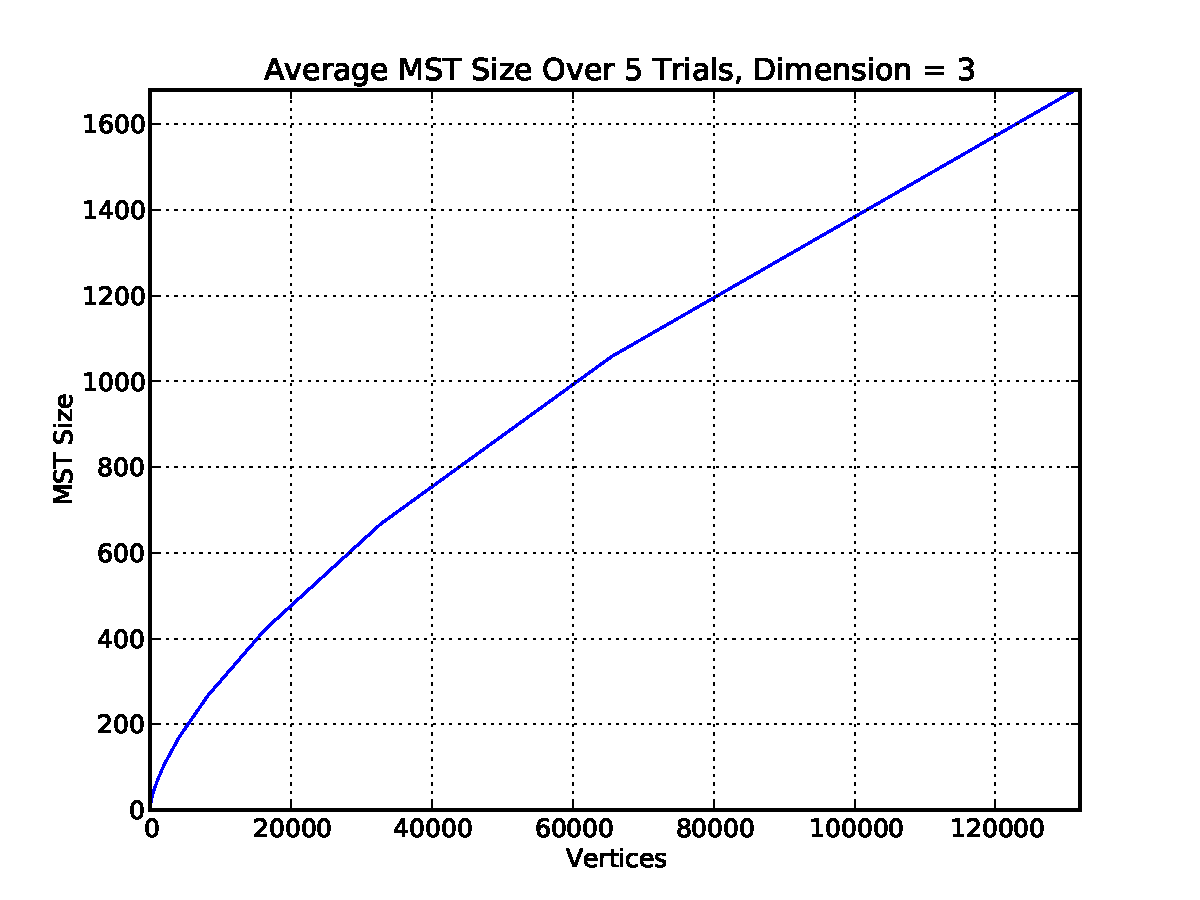
\includegraphics[scale=0.6]{graphs/kruskals-dimension-3.pdf}
\begin{tabular}{ | r | l |}
\hline
\bf{\itshape{n}} & \bf{Avg. MST Weight} \\
\hline
16 & 4.566855 \\
\hline
32 & 6.925250 \\
\hline
64 & 11.133249 \\
\hline
128 & 17.818338 \\
\hline
256 & 27.646692 \\
\hline
512 & 43.728298 \\
\hline
1024 & 68.244339 \\
\hline
2048 & 107.170555 \\
\hline
4096 & 168.915375 \\
\hline
8192 & 266.453552 \\
\hline
16384 & 422.085632\\
\hline
32768 & 667.827393\\
\hline
\end{tabular}
\end{center}

This curve is best described by a function of the form $f(n)=an^b$, where $a > 0$ and $\frac{1}{2} \leq b \leq 1$. Using Mathematica's {\tt FindFit} function in conjunction with the data used to generate the above graph, we achieved $a=0.68055$ and $b=0.662729$ as the best fit values for this function, giving us the following best guess for $f(n)$:
\[f(n) \approx 0.68n^{\frac{2}{3}}\]

\pagebreak

\subsection*{Dimension 4 - Hypercube}

The following is a graph showing the average tree size over 5 trials for several values of $n$:
\begin{center}
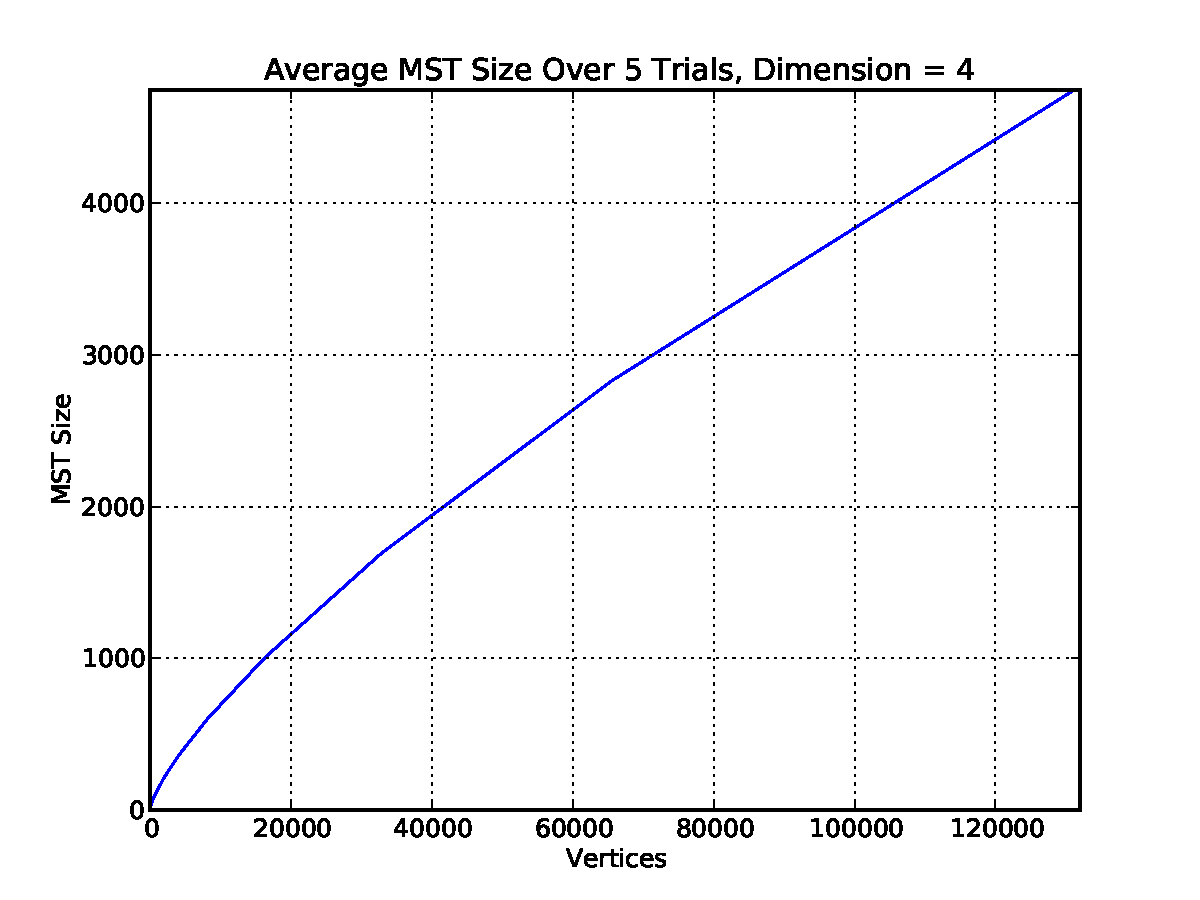
\includegraphics[scale=0.6]{graphs/kruskals-dimension-4.pdf}
\begin{tabular}{ | r | l |}
\hline
\bf{\itshape{n}} & \bf{Avg. MST Weight} \\
\hline
16 & 6.159772 \\
\hline
32 & 10.294616 \\
\hline
64 & 17.242434 \\
\hline
128 & 28.670132 \\
\hline
256 & 47.566528 \\
\hline
512 & 78.802025 \\
\hline
1024 & 129.762085 \\
\hline
2048 & 217.340424 \\
\hline
4096 & 361.436401 \\
\hline
8192 & 602.498047 \\
\hline
16384 & 1007.845337 \\
\hline
32768 & 1688.796265 \\
\hline
\end{tabular}
\end{center}

This curve is best described by a function of the form $f(n)=an^b$, where $a > 0$ and $\frac{1}{2} \leq b \leq 1$. Using Mathematica's {\tt FindFit} function in conjunction with the data used to generate the above graph, we achieved $a=0.744403$ and $b=0.74331$ as the best fit values for this function, giving us the following best guess for $f(n)$:
\[f(n) \approx 0.74n^{\frac{3}{4}}\]

\section*{Discussion}
\subsection*{Choice of Algorithm}
\hspace{5mm} We decided to use Kruskal's algorithm instead of Prim's algorithm because we wanted to work with something new. We both implemented heaps (priority queues) last year in CS51, and Matt implemented Prim's algorithm for his CS51 project. In addition, we felt that the programming work required to fully implement Kruskal's algorithm would parallelize better than the work required to implement Prim's algorithm. That is, we thought our mutual time would be better spent implementing a disjoint set library, an efficient sort procedure, and the pseudocode for Kruskal's than it would be implementing a heap and the pseudocode for Prim's.

\subsection*{Implementation Details}
\hspace{5mm} Our code is subdivided into the following files: \texttt{graph.c} \& \texttt{graph.h}, in \texttt{disjoint-set.c} \& \\\texttt{disjoint-set.h}, and \texttt{main.c}.

\texttt{graph.h} declares \texttt{structs} for edges, graphs, and test graphs and \texttt{graph.c} provides implementations of helper functions for working with these \texttt{struct}s (i.e., generating graphs, sorting edges, etc.). Vertices are represented by a unique integer in the range [0, \texttt{numpoints}). Edges consist of two vertices (\texttt{u} and \texttt{v}) and a weight. Graphs are implemented as edge lists (arrays), since the crux of Kruskal's algorithm involves iterating through a sorted list of edges, and this implementation was the easiest to interface with for this purpose. Test graphs are stored in \texttt{test\_graphs struct}, which contain two parallel arrays - an array of graphs and a matching array of pre-calculated minimum MST weights for checking the correctness of an MST algorithm.

\texttt{disjoint-set.h} declares a disjoint set forest \texttt{struct} for working with disjoint sets and\\ \texttt{disjoint-set.c} implements
the appropriate functions for disjoint sets (i.e. union, find, make set).

\texttt{main.c} contains our implementation of Kruskal's and the code for processing the command line arguments and running the appropriate functions.

All of the above files are heavily commented if more information is desired.

\subsubsection*{Pseudorandom Number Generator}
\hspace{5mm} We seeded our pseudorandom number generator (PRNG) using the system clock. We had one interesting issue for smaller values of $n$ where the PRNG was not reseeded for runs completed in quick succession, since the system clock had not updated itself between runs. This is because we had originally seeded the PRNG when generating graphs. Because our code allows for multiple runs (to average the results), and each graph generation was seeding the PRNG, if a run was fast enough, the next graph generation might reseed the PRNG with the same value leading to the same random sequence of numbers. To avoid this we simply seed the PRNG once, before any of the runs in \texttt{main.c}.

\subsection*{Optimization}
\hspace{5mm} In order to handle large $n$, we simplified the graph by discarding heavy edges unlikely to be included by Kruskal's algorithm in the MST. We derived our definition of what constitutes a 	``heavy" edge by running our program for $n$ equal to powers of 2 through 8192 for each dimension (0, 2, 3, and 4) and logging the heaviest edge included in the MST each time.\footnote{Passing {\tt randmst} the flag 3 will cause it to print out the heaviest edge in the MST.} We picked a threshold weight based on these data which we then used to decide whether or not an edge should be included in the array sorted by Kruskal's algorithm during each run. This sort is the slowest part of Kruskal's, and decreasing the number of edges we need to sort consequently accelerates the execution time of Kruskal's. Discarding edges in this manner will never lead to a situation where the program returns the wrong tree because we are truncating the array that Kruskal's pulls edges from at a point beyond that needed by the algorithm to construct an MST. That is, we are throwing out edges we know will never be used. As such, our optimized program must give the same result as a non-optimized program.

\subsubsection*{Memory}
\hspace{5mm} Prior to the above optimization we would run out of memory with which to store the edge lists for generated graphs. The optimization allows us to store much fewer edge weights, and by dynamically resizing the edge list array as necessary when building up a graph, we are able to use significantly less memory. Thus, the optimization helps not only in running time but also space complexity.

\subsection*{Growth Rates}
\hspace{5mm} We were most surprised by the growth rate of the size of the MST for dimension 0. We had not expected a constant function to describe the growth of any of the dimensions. We can explain this constant growth function by noting that as the number of nodes and edges in the graph increases exponentially, the number of extremely light edges available to the algorithm to include in an MST also increases exponentially. This idea is key to understanding the growth of the MSTs for the other dimensions. It also explains why our optimization by truncation works well, since it suggests that we are throwing out an increasing number of unnecessary edges.

We were also surprised to see, for dimensions 2, 3, and 4, how the value of the constant $b$ appears to be approximately equal to $\frac{\text{dimension - 1}}{\text{dimension}}$. Furthermore, $a$ seems to approach $b$ as the number of dimensions increases, converging to a formula of the form:
\[
f(n) = \dfrac{d-1}{d}n^{\frac{d-1}{d}} \text{where $d$ is the \# of dimensions}
\]
\hspace{5mm} We are not sure if this trend holds for higher values of $d$, but it is certainly worth noting. If this trend does hold it suggests that as the number of dimensions approaches infinity, the function approaches $f(n) = n$. Since an MST must contain $n - 1$ edges to connect all vertices, this indicates that the average edge weight in an MST as $d$ approaches infinity is approximately 1. It is hard to reason about what this means in the context of infinite dimensional space since it is hard to reason about infinite dimensional space. This is all dependent on the above trend continuing for higher and higher values of $d$.
\subsection*{Runtime}
\hspace{5mm} On average, our program (graph generation \emph{and} Kruskal's) takes under 10 seconds to complete a single run on a graph for which $n = 40000$ for all dimensions. On average, our program takes 90 seconds to complete a single run on a graph where $n = 2^{17} = 131072$ for dimension 0, and X seconds for dimension 4. Given our optimization via truncation, these runtimes make sense. We did not notice the cache size of our computers having an effect on our runtime.


\end{document}



